\documentclass{standalone}
\usepackage{tikz}
\usetikzlibrary{arrows.meta}

\begin{document}

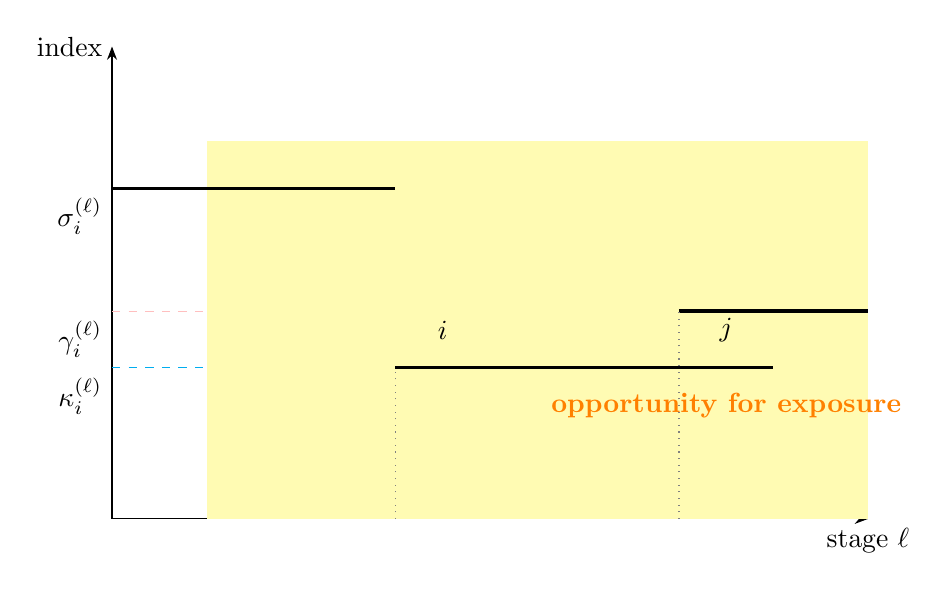
\begin{tikzpicture}[scale=1.2]

    % Axes
    \draw[-Stealth] (0,0) -- (8,0) node[below] {stage $\ell$};
    \draw[-Stealth] (0,0) -- (0,5) node[left] {index};

    % Horizontal dashed lines for indices
    \draw[dashed, cyan] (0,3.5) -- (7,3.5) node[right, black] {$\sigma_i^{(\ell)}$};
    \draw[dashed, pink] (0,2.2) -- (7,2.2) node[right, black] {$\gamma_i^{(\ell)}$};
    \draw[dashed, cyan] (0,1.6) -- (7,1.6) node[right, black] {$\kappa_i^{(\ell)}$};

    % Vertical dashed lines indicating stages
    \draw[dashed, cyan] (3,0) -- (3,3.5);
    \draw[dashed, cyan] (6,0) -- (6,1.6);

    % Shaded yellow regions
    \fill[yellow!30] (1,0) rectangle (5,4); % Left shaded region
    \fill[yellow!30] (5,0) rectangle (8,4); % Right shaded region

    % Text labels within shaded regions
    \node at (3.5, 2) {\textbf{$i$}}; % Left region label
    \node at (6.5, 2) {\textbf{$j$}}; % Right region label

    % Annotations
    \node[orange] at (6.5, 1.2) {\textbf{opportunity for exposure}};

    % Black horizontal bars
    \draw[very thick, black] (0,3.5) -- (3,3.5);
    \draw[very thick, black] (3,1.6) -- (7,1.6);
    \draw[very thick, black] (6,2.2) -- (8,2.2);

    % Additional dashed lines for clarification
    \draw[dotted, gray] (3,0) -- (3,1.6);
    \draw[dotted, gray] (6,0) -- (6,2.2);

    % Labels for minimum indices
    \node[below left] at (0,3.5) {$\sigma_i^{(\ell)}$};
    \node[below left] at (0,2.2) {$\gamma_i^{(\ell)}$};
    \node[below left] at (0,1.6) {$\kappa_i^{(\ell)}$};

\end{tikzpicture}

\end{document}